\section{Dynamic games}

\Que{What is a dynamic game?}
\Ans[A dynamic game]{ is a game in which players moves are sequential and not simultaneous.}
\Spec{They can be of \textbf{perfect information} (meaning that every player can do every decision with full awareness) or \textbf{imperfect information} (meaning some decisions are “simultaneous” or Nature moves).

We have two scenarios for the former information:
\begin{itemize}
    \item \textbf{endogenous uncertainty}: information sets contain multiple nodes (simultaneous moves)
    \item \textbf{exogenous uncertainty}: there is a choice of Nature (lotteries)
\end{itemize}}

\Que{How can we represent dynamic games?}
\Ans[]{Graphically, they can be represented as a tree, where each level is a move and each node is the response to a specific opponent' move.
\begin{figure}[!ht]
    \centering
    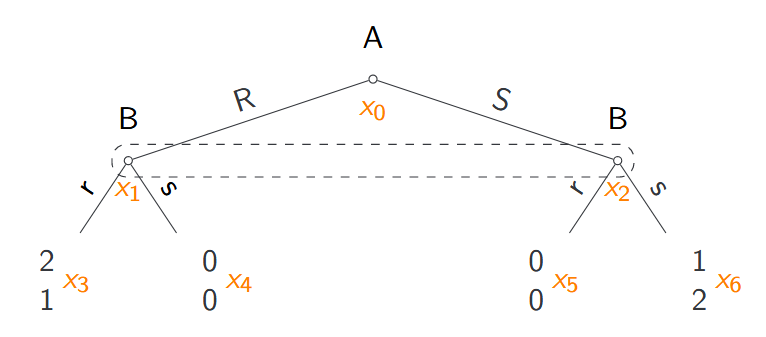
\includegraphics[width=0.5\linewidth]{dynamicTree.png}
\end{figure}
Dotted circle (or just a dotted arch) shows node from the same information set, i.e. the game stage a player can have.

A \textbf{information set} $h_i$ is a mathematical representation of player's possible moves. If $h_i = \{x_j\}$ (i.e. it has just one node), then the node is fully aware of previous moves.}

\Que{How to define a strategy in dynamic games?}
\Ans[]{A strategy in dynamic games need to account for the history of play.

Imagine a two-move game, B has strategy \m{s_B = (a_1, a_2)} where $a_1$ is the response to A playing move 1. If the match is played twice, B has strategy \mat{s_B = (a_1, a_{11}, a_{12}, a_{21}, a_{22})}, where $a_11$ is the answer of A first move, B playing 1 and A answering with 1 (for example, \m{s_b = (1,1,1,1,1)} means B playing 1 no matter what. Instead, \m{s_b = (1,2,1,1,1)} means B playing 2 if A's second move is 1, otherwise playing 1.}